\documentclass[12pt, letterpaper,spanish]{article}
\usepackage[letterpaper]{geometry}
\usepackage[T1]{fontenc} %para escribir con caracteres utf8 como tildes
\usepackage[utf8]{inputenc} %para escribir con caracteres utf8 como tildes
\usepackage[spanish]{babel} %para escribir con caracteres utf8 como tildes
\usepackage{lmodern} % latin modern font
\usepackage{color}
\usepackage[svgnames]{xcolor} % para hacer enfasis con colores
\usepackage{amssymb}
\usepackage{amsmath}
\usepackage{hyperref}
\usepackage{multirow}
\usepackage{array}
\usepackage{mathtools} % para el modulo
\DeclarePairedDelimiter\abs{\lvert}{\rvert}%
\DeclarePairedDelimiter\norm{\lVert}{\rVert}%
\hypersetup{
	colorlinks=true,
	linkcolor=black,
	filecolor=magenta,      
	urlcolor=cyan,
}

\usepackage{listings}
\definecolor{background}{rgb}{0.39, 0.40, 0.34}
\definecolor{keywords}{rgb}{1.0, 0.0, 0.5}
\definecolor{comments}{rgb}{0.75, 0.75, 0.75}
\definecolor{strings}{rgb}{0.91, 0.84, 0.42}
\definecolor{names}{rgb}{0.4, 1.0, 0.0}
\definecolor{white}{rgb}{1.0, 1.0, 1.0}
\definecolor{types}{rgb}{0.13, 0.67, 0.8}
\definecolor{numbers}{rgb}{0.54, 0.17, 0.89}

\lstdefinelanguage{PSharp}{
	keywords={method, void},
	keywordstyle=\color{keywords}\bfseries,
	ndkeywords={int},
	ndkeywordstyle=\color{types}\bfseries,
	identifierstyle=\color{white},
	sensitive=false,
	emph={print},
	emphstyle=\color{names},
	comment=[l]{//},
	morecomment=[s]{/*}{*/},
	commentstyle=\color{comments}\ttfamily,
	stringstyle=\color{strings}\ttfamily,
	morestring=[b]',
	morestring=[b]"
}

\lstset{
	language=PSharp,
	backgroundcolor=\color{background},
	extendedchars=true,
	basicstyle=\footnotesize\ttfamily,
	showstringspaces=false,
	showspaces=false,
	numbers=left,
	numberstyle=\footnotesize,
	numbersep=9pt,
	tabsize=2,
	breaklines=true,
	showtabs=false,
	captionpos=b
}


\usepackage{amsthm} % para teoremas y lemas
\usepackage{graphicx} % para imagenes
\usepackage{titling} % para el pretitle
\usepackage{clrscode3e} % para pseudocodigos
\usepackage[stable]{footmisc} % para permitir footnotes in los encabezados

%\usepackage[cache=false]{minted} %para representar los codigos necesita config extra
%\renewcommand\theFancyVerbLine{\normalsize\arabic{FancyVerbLine}} % incrementar el tamaño de linenumbers de minted


\newtheorem{theorem}{Teorema}[subsection]
\newtheorem{corollary}{Corolario}[theorem]
\newtheorem{lemma}{Lema}[subsection]
\newtheorem{lemmacorollary}{Corolario}[lemma]
\theoremstyle{definition}
\newtheorem*{definition}{Definición}
\theoremstyle{remark}
\newtheorem*{remark}{Observación}
\renewcommand{\qedsymbol}{$\blacksquare$} % se remplaza el simbolo vacio de final de demostración
\graphicspath{ {./_static/} }

%--------------------------
% NO MODIFICAR ESTE DOCUMENTO
%--------------------------
	
\begin{document}
	
\begin{titlepage}
	\begin{center}
		
\includegraphics[width = 3cm]{escudoUH} 
	\end{center}
	\begin{center}
		Universidad de La Habana \\\vspace{0.2cm} Facultad de Matemática y Computación
	\end{center}
	\centering
	\vspace{1cm} \par
	{\scshape\Large Proyecto de Compilación + Intenteligencia Artificial + Simulación\par}
	\vspace{5mm} \par
	{\scshape\Huge Simulador de un Jefe Técnico de MotoGP\par}
	\vspace{5mm} \par
	\vfill
	{\Large \textbf{Autores:} \par}
	{\large Arnel Sánchez Rodríguez \space Grupo: C312 \par}
	\href{mailto:arnelsanchezrodriguez@gmail.com}{arnelsanchezrodriguez@gmail.com}\par
	\vspace{3mm} \par
	{\large Samuel Efraín Pupo Wong \space Grupo: C312 \par}
	\href{mailto:s.pupo@estudiantes.matcom.uh.cu}{s.pupo@estudiantes.matcom.uh.cu}
	\vspace{3mm} \par
	{\large Darián Ramón Mederos \space Grupo: C312 \par}
	\href{mailto:darianrm24@gmail.com}{darianrm24@gmail.com}
	\vspace{3mm} \par
	\vfill
	{\Large 2021-2022 \par}
\end{titlepage}	
\pagebreak
\tableofcontents
\pagebreak
\section{Motociclismo de Velocidad}
	El motociclismo de velocidad es una modalidad deportiva del motociclismo disputada en circuitos de carreras pavimentados. Las motocicletas que se usan pueden ser prototipos, es decir desarrolladas específicamente para competición, o derivadas de modelos de serie (en general motocicletas deportivas) con modificaciones para aumentar las prestaciones. En el primer grupo entran las que participan en el Campeonato Mundial de Motociclismo, y en el segundo las Superbikes, las Supersport y las Superstock.
	
	Las motocicletas deben presentar una serie de características como son estabilidad, alta velocidad (tanto en recta como en paso por curva), gran aceleración, gran frenada, fácil maniobrabilidad y bajo peso.
	
	\begin{center}
		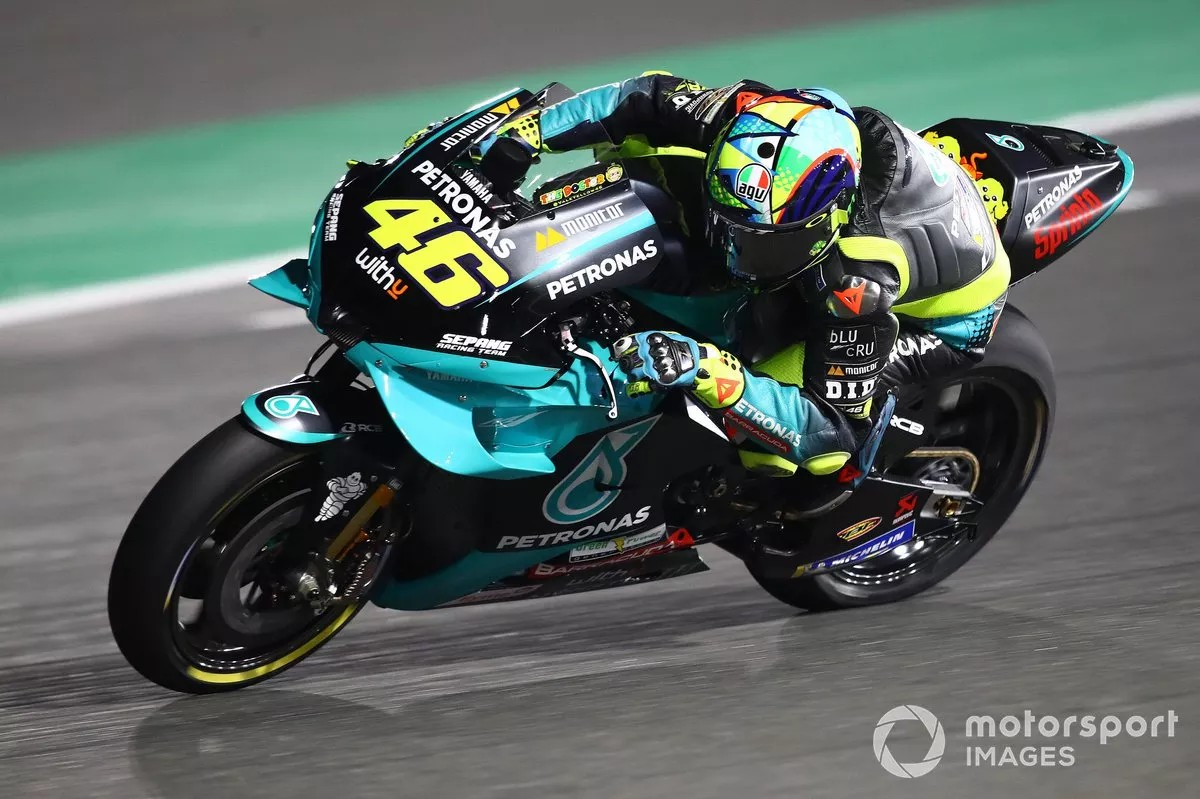
\includegraphics[width = 12cm]{imagen1} 
	\end{center}	
	
\section{Estructura del Paddock}
	El \textbf{Jefe Técnico} de cada estructura se configura como una personalidad de bastante importancia dentro de un box, pues es quién se encarga de dirigir y controlar que todo funcione como un excelente engranaje que gane carreras. De igual importancia es la telemetría dentro de un box en MotoGP. Al fin y al cabo, los \textbf{Ingenieros Telemétricos} son las personas que se encargan de analizar, leer y comprender todos los datos proporcionados por el piloto, así como transmitirselos en boca al protagonista. Se trata de una figura de la que depende mucha de la información acerca de cualquier cambio realizado en la moto o asumir los puntos más fuertes de sus pilotos. Los \textbf{Mecánicos} también desempeñan un papel fundamental a la hora de construir la máquina perfecta.

\section{Pista}
	Se utilizará como referencia el circuito de Misano, Misano World Circuit Marco Simoncelli, autódromo localizado en la fracción de Santa Mónica, comuna de Misano Adriático (provincia de Rímini), región de Emilia-Romaña, Italia. 
	
	\begin{center}
		\includegraphics[width = 12cm]{circuito} 
	\end{center}
	
\section{Definición del Problema}
	Existirán varios pilotos con sus respectivas motos, las cuáles difieren entre sí en cuanto a sus prestaciones. Cada piloto posee su propio método de manejo, siendo algunos más cuidadosos y otros más agresivos. La pista se encuentra influenciada por el accionar del clima, puesto que no es lo mismo el manejo durante un día soleado que bajo la lluvia. Por tanto, el resultado de un piloto se verá condicionado por su moto, su modo de conducción y el clima.\par
	Sin embargo, durante la carrera las condiciones pueden variar y el Jefe Técnico será el encargado de señalar los ajustes necesarios que el piloto deberá hacer para mejorar su rendimiento. Dicho intercambio de información se hará al finalizar cada vuelta utilizando un lenguaje imperativo, mediante el uso de palabras claves para que el piloto no necesite analizar situaciones complejas y pueda concentrarse en pilotar de la forma mas eficiente posible.\par
	De esta manera, la simulación de la carrera será dinámica, puesto que entre las vueltas podrán existir variaciones provocadas por los ajustes propuestos por el Jefe Técnico, el cuál podrá ser una persona o una IA.\par
	
\section{Definición del Lenguaje}
	\include{DefiniciónDelLenguaje.tex}
\end{document}

